% Intended LaTeX compiler: pdflatex
\documentclass{scrartcl}
    \usepackage{amsmath, amssymb, bm}
		\usepackage[utf8]{inputenc}
		\usepackage[dvipdfmx]{graphicx}
		\usepackage[dvipdfmx]{color}
		\usepackage[backend=biber,bibencoding=utf8]{biblatex}
		\usepackage{url}
		\usepackage{indentfirst}
		\usepackage[normalem]{ulem}
		\usepackage{longtable}
		\usepackage{minted}
		\usepackage{fancyvrb}
    \usepackage[dvipdfmx,colorlinks=false,pdfborder={0 0 0}]{hyperref}
    \usepackage{pxjahyper}
    \usepackage{caption}
\author{情報科学類二年 江畑 拓哉(201611350)}
\date{}
\title{ヒューマンインタフェース第一回レポート}
\begin{document}

\maketitle

\section{身近な道具、家電製品、コンピュータやその部品などからBadUI/GoodUIであるものを調査して、一つ報告せよ。}
\label{sec:org848d7db}
また、その問題点/良い点を考察し、解決策/使われている方策とともに論ぜよ。これまでに講義内で扱った言葉と概念を駆使して論ずること。\\

Amazon(\url{https://www.amazon.co.jp})を GoodUI として調べた。\\
このサイトにアクセスして始めに目に付くのはおそらくバナー広告だろう。ここには割引などのユーザにとって有益となる情報が載せられている。Amazonは必ずしも買うものを決めた状態で開くサイトではないという点(例えば現実で当てもなく百貨店を散策するような気分でここに訪れることがあるはずだ)を考えれば、ここに所謂``お得情報''があることはユーザにとっては必ずしも障害になるものではないはずだ。また、このバナー広告は(目立つようにこの部分だけは、とも考えられる)自動でスライドするため眺めているだけでもウィンドウショッピングのそれを体験することが出来る。\\
そしてもし素直に検索を行いたいと思ってほんの少しでも視線を動かせば、その上にある検索欄に目がゆくはずだ。濃色と淡色ではっきりと強調されるだけでなく、検索ボタンに周囲の藍色の補色に近いオレンジを採用していることで、この項目は極めて目立つ。これは同じ位置にあるカート欄も同様で、かつて自分が何を買おうとしていたかをはっきりと確認することが出来る。\\
そして次に目に入るのがフラットデザインのカテゴリ・注文履歴などである。これらは極力先述の注目度を殺さないように設計されているようで、特に検索欄周辺の濃色に対して淡色を採用している。またカテゴリごとに色分けをしているため、ユーザは無意識的に目に入るそれであっても何度もアクセスをすることでどのカテゴリがどの色であるかを何気なく理解することが出来る。これによってカテゴリにアクセスしたい場合にはその名称を毎回目で探す必要がなく、ぱっと目に入った色情報からそれぞれにアクセスすることが出来る。\\
フラットデザインはかつて猛威を振るっていたアニメーションや立体表現などの動的で派手なデザインに対して地味に見えるかも知れないが、自然で落ち着いた印象がある。\\
このように視覚的にわかりやすいデザインはアフォーダンスがわかりやすいと言えるだろう。\\
以上を見終わって更にスクロールすれば最近 Amazon が追加した目玉機能の一つであるダッシュボタンが顔を見せる。これはいつも買っている品物を再び買いたいというゴールに対し詳細化、実行のコストを最小にすることが出来る。\\
最後に購入を行うために``カートに入れる''ボタンを押した場合に、ヘッダのカート欄にあるこれまでカートに入れた品物の個数が更新される点は、適切なフィードバックと言えるだろう。\\
これらのことから、Amazon は GoodUI と言える。\\


\begin{figure}[htbp]
\centering
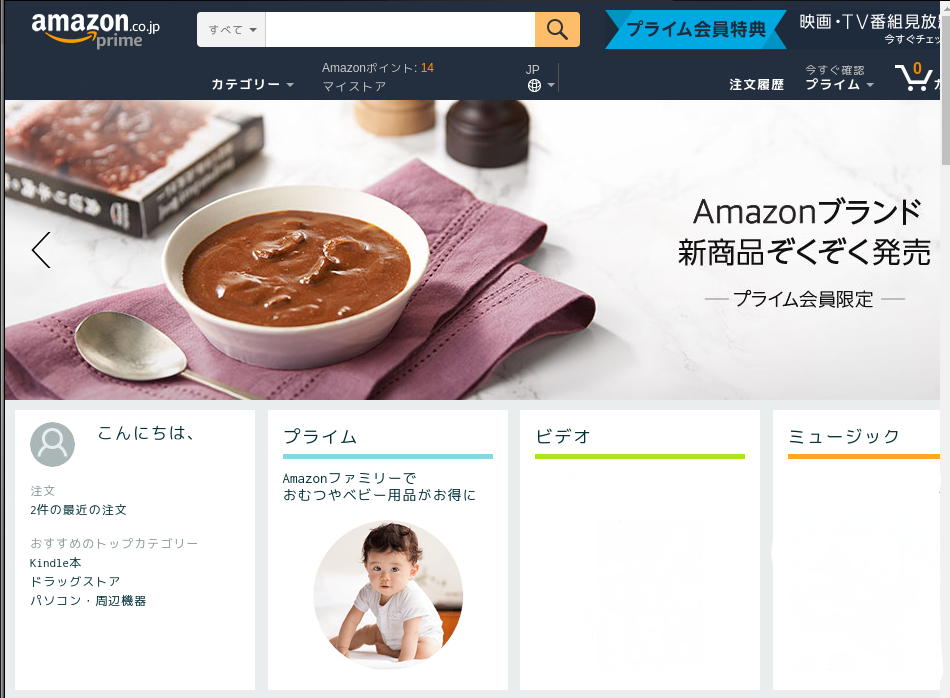
\includegraphics[width=0.5\linewidth]{./Screenshot1.png}
\caption{ホーム画面}
\end{figure}

\begin{figure}[htbp]
\centering
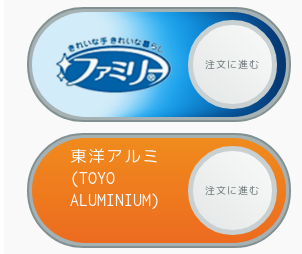
\includegraphics[width=0.5\linewidth]{./Screenshot2.png}
\caption{ダッシュボタン}
\end{figure}
\end{document}
